\documentclass[12pt]{article}

\usepackage{geometry}
\geometry{letterpaper, margin=1in}
\usepackage{graphicx}
\usepackage{amsmath}
\usepackage{natbib}
\usepackage{authblk}
\usepackage{tablefootnote}
\usepackage{pgfplots}

\pgfplotsset{compat=1.17}

\definecolor{tab_blue}{rgb}{0.1216, 0.4667, 0.7059}
\definecolor{tab_orange}{rgb}{1.0000, 0.4980, 0.0549}
\definecolor{tab_grey}{rgb}{0.4980, 0.4980, 0.4980}
\definecolor{tab_red}{rgb}{0.8392, 0.1529, 0.1569}
\definecolor{tab_brown}{rgb}{0.5490, 0.3373, 0.2941}
\definecolor{tab_purple}{rgb}{0.5804, 0.4039, 0.7412}

\usepackage{xr}
\makeatletter
\newcommand*{\addFileDependency}[1]{% argument=file name and extension
  \typeout{(#1)}% latexmk will find this if $recorder=0 (however, in that case, it will ignore #1 if it is a .aux or .pdf file etc and it exists! if it doesn't exist, it will appear in the list of dependents regardless)
  \@addtofilelist{#1}% if you want it to appear in \listfiles, not really necessary and latexmk doesn't use this
  \IfFileExists{#1}{}{\typeout{No file #1.}}% latexmk will find this message if #1 doesn't exist (yet)
}
\makeatother

\newcommand*{\myexternaldocument}[1]{%
    \externaldocument{#1}%
    \addFileDependency{#1.tex}%
    \addFileDependency{#1.aux}%
}

\myexternaldocument{main}

% Custom numbering for SI
\newcommand{\beginsupplement}{
    \setcounter{section}{0}
    \renewcommand{\thesection}{S\arabic{section}}
    \setcounter{equation}{0}
    \renewcommand{\theequation}{S\arabic{equation}}
    \setcounter{table}{0}
    \renewcommand{\thetable}{S\arabic{table}}
    \setcounter{figure}{0}
    \renewcommand{\thefigure}{S\arabic{figure}}}

\title{Journal of Aerosol Science\\ \large Supporting Information for: Differences and similarities in optical properties of coated fractal soot and its surrogates}

\author[1]{Egor Demidov}
\author[2,5]{Ogochukwu Y. Enekwizu}
\author[1,4]{Ali Hasani}
\author[3]{Chong Qiu}
\author[1,2]{Alexei F. Khalizov}

\affil[1]{Department of Chemistry and Environmental Science, New Jersey Institute of Technology, Newark, NJ 07102, USA}
\affil[2]{Department of Chemical and Materials Engineering, New Jersey Institute of Technology, Newark, NJ 07102, USA}
\affil[3]{Department of Chemical Engineering, University of New Haven, West Haven, CT 06516, USA}
\affil[4]{Now at: Center for Devices and Radiological Health, U.S. FDA}
\affil[5]{Now at: Brookhaven National Laboratory, Upton NY 11973}

% Remove date
\date{}

\renewcommand\Affilfont{\small}

\begin{document}
\maketitle

\tableofcontents
\listoffigures
\newpage

\beginsupplement

\section{Aerosol classification by DMA and APM}

The DMA operates by classifying charged particles based on their mobility in an electric field. A specific applied voltage corresponds to a particular electrical mobility diameter of particles, $D$, transmitted by the instrument, and the relationship is defined by equation \ref{s:eq:dma},

\begin{equation}
    \frac{D}{C_C}=\frac{2n_eeVL}{3\eta q_{sh}\ln{\frac{r_2}{r_1}}}
    \label{s:eq:dma}
\end{equation}

\noindent where $C_C$ is the Cunningham slip correction factor, $n_e$ is the number of elementary charges, $V$ is the set voltage between electrodes, $L$, $r_1$, $r_2$ are parameters related to the geometry of the instrument, $\eta$ is the gas kinematic viscosity, and $q_{sh}$ is the sheath flow through the DMA. $C_C$ is a function of particle diameter \citep{davies1945definitive}, where $\ell$ is the mean free path of gas, and significantly deviates from unity for our particle size range,
\begin{equation}
    C_C=1+2\frac{\ell}{D}\left(1.254+0.4e^{-1.1\frac{D}{2\ell}}\right)
    \label{s:eq:cunningham}
\end{equation}
The APM operates by applying an electric field to particles passing in a flow of gas through a gap between revolving cylindrical electrodes. Mass is only proportional to particle charge at a constant voltage and revolution speed (Equation \ref{s:eq:apm}),
\begin{equation}
    mr\omega^2=q\frac{V}{r\ln{\frac{r_2}{r_1}}}
    \label{s:eq:apm}
\end{equation}
where $q$ is the total charge on a particle, $r$, $r_1$, $r_2$ are the geometric parameters of the instrument, and $V$ is the set voltage. Figure \ref{s:fig:smps} shows size distributions of all aerosols considered in this study as normalized number concentration versus electrical mobility diameter. The size distribution was obtained with a Scanning Mobility Particle Sizer (SMPS) system, consisting of an electrostatic classifier and a CPC. Figure \ref{s:fig:apm-bare-nigrosin} shows mass distributions of nigrosin of different electrical mobility diameters.

\begin{figure}[htp]
\centering
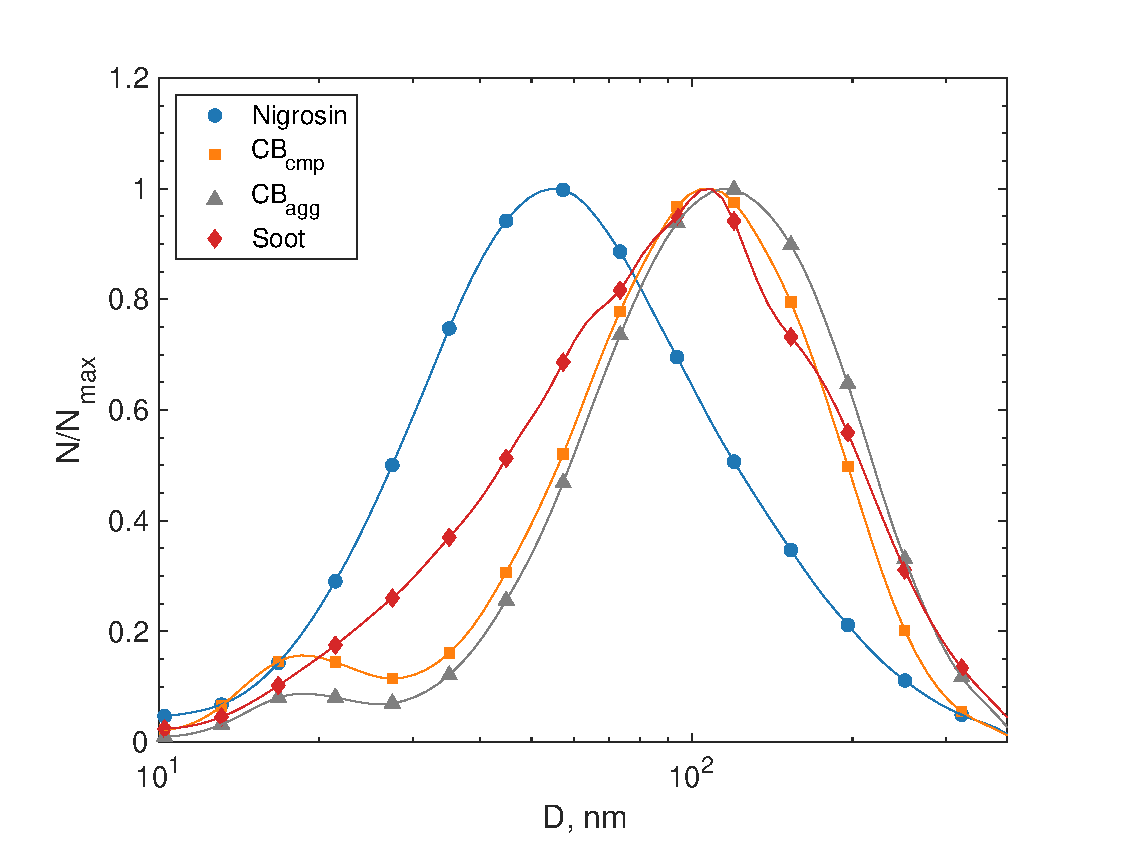
\includegraphics[scale=0.7]{images/fig_supp_smps.eps}
\caption{Size distributions of nigrosin, compact CB, agglomerated CB, and flame soot (markers at every 5\textsuperscript{th} point)}
\label{s:fig:smps}
\end{figure}

\begin{figure}[htp]
    \centering
    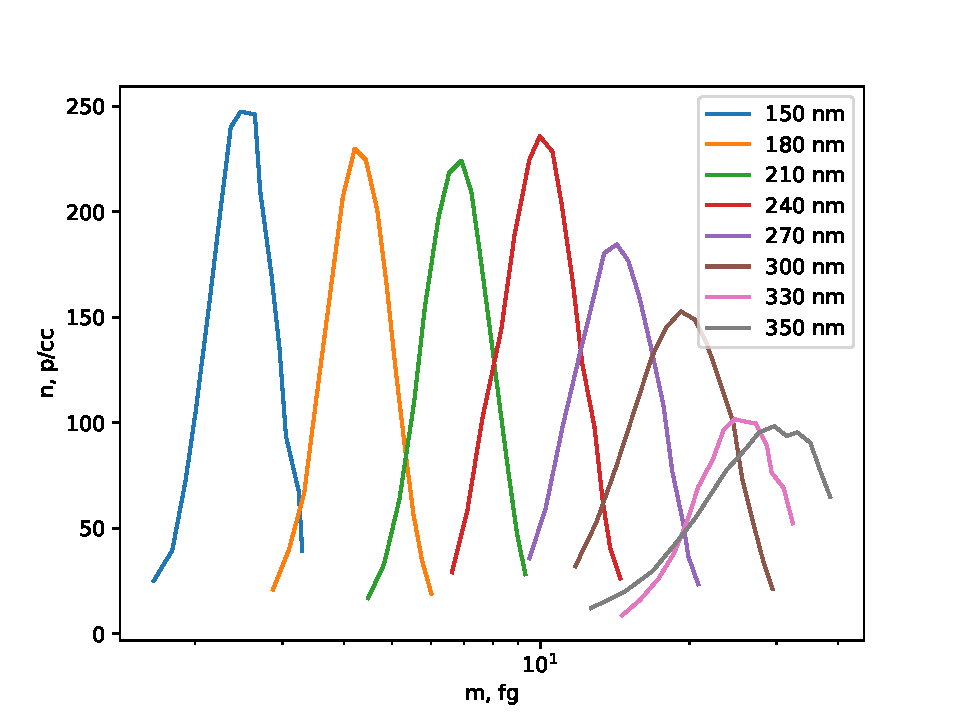
\includegraphics[width=0.8\textwidth]{images/apm-bare-nigrosin.pdf}
    \caption{Mass distributions of nigrosin of different mobility diameters}
    \label{s:fig:apm-bare-nigrosin}
\end{figure}

\section{Multiple charging}
\subsection{Charging probabilities}
An aerosol particle carrying two charges will not have twice the electrical mobility diameter of a singly charged particle because the diameter is proportional not only to the number of elementary charges $n_e$, but also to the Cunningham slip correction factor, $C_C$.

\begin{equation}
    \frac{D_1}{D_2}=\frac{n_{e,1}C_{C,1}}{n_{e,2}C_{C,2}}
\end{equation}

\noindent There are two ways to determine the number fraction of particles carrying different charges. One way is to calculate it from the size distribution (a.k.a. a DMA scan) and charging probability of each particle size \citep{RN10}. Another approach is to pass size-classified aerosol through another charger, where most of the multiply charged particles will become singly charged. When taking a size distribution with the second DMA, the true electrical mobility diameter of those particles will be revealed and the doubly charged particles will be separated from the singly charged particles. By calculating the areas under each particle mode, we can estimate the fractions of singly and doubly charged particles in the aerosol.

Figure \ref{s:fig:probability} shows the charging probabilities for different number of charges as a function of the electrical mobility diameter of the particles. The probabilities were calculated using the method described in \citep{RN10}. The number fraction of doubly charged particles can be calculated from the size distribution and charging probabilities:

\begin{equation}
    f_2=\frac{N|_{D=D_2}\cdot p|_{D=D_2}}{N|_{D=D_1}\cdot p|_{D=D_1}+N|_{D=D_2}\cdot p|_{D=D_2}}
\end{equation}

\begin{figure}[htp]
\centering
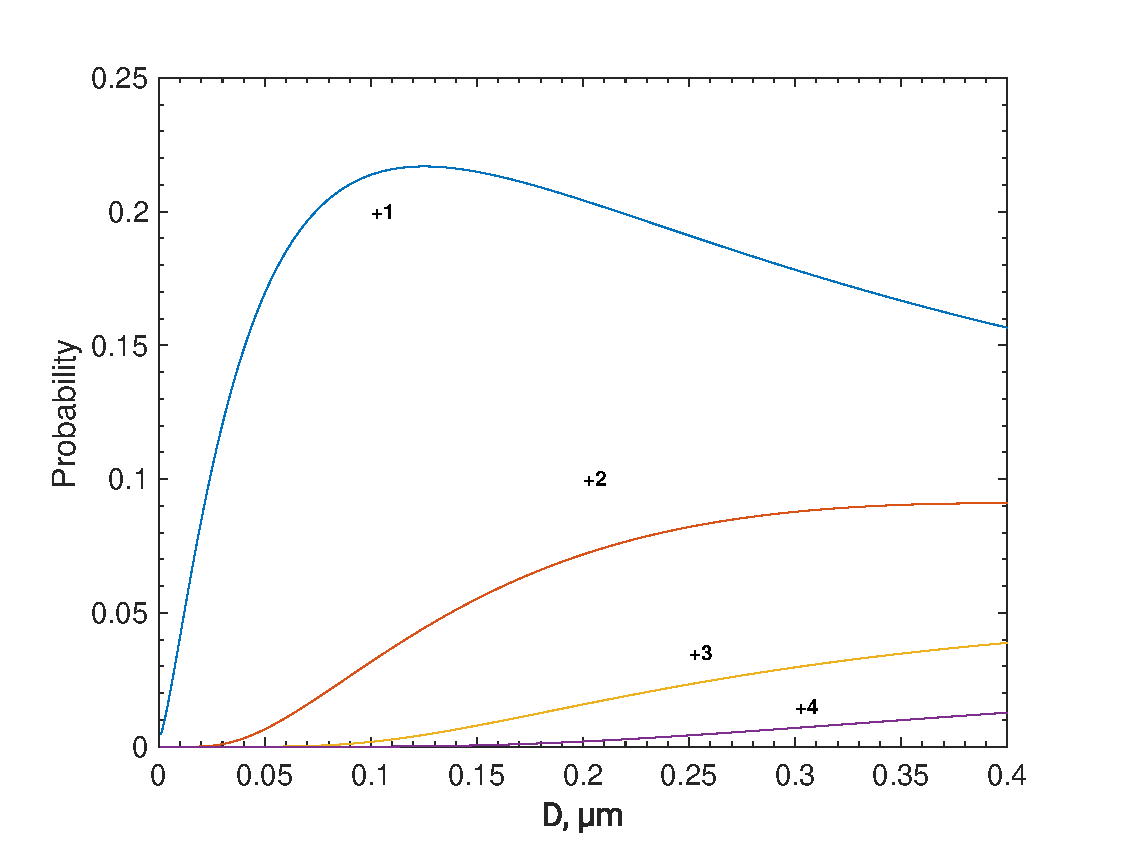
\includegraphics[scale=0.7]{images/fig_supp_probability.eps}
\caption{Charging probability of aerosol versus mobility diameter, figure produced using the data of \citet{RN10}}
\label{s:fig:probability}
\end{figure}

\subsection{Quantifying multiply charged particles via recharging}

Figure \ref{s:fig:tdma} shows a recharged tandem DMA (TDMA) scan of 150 nm nigrosin, where size-classified aerosol is recharged with a second bipolar charger and a size distribution scan is performed by the second DMA. Recharging causes the majority of doubly and triply charged particles to become singly charged and reveals those particles as separate peaks (indicated by $2\rightarrow 1$ and $3\rightarrow 1$ in the figure). Recharging also causes some particles that were initially singly charged to attain double and triple charges (peak indicated by $1\rightarrow 2$ and $1\rightarrow 3$ in the figure). Particles that retain single charges after recharging are indicated with $q\rightarrow q$. The number of triply charged particles is typically small.

\begin{figure}[htp]
\centering
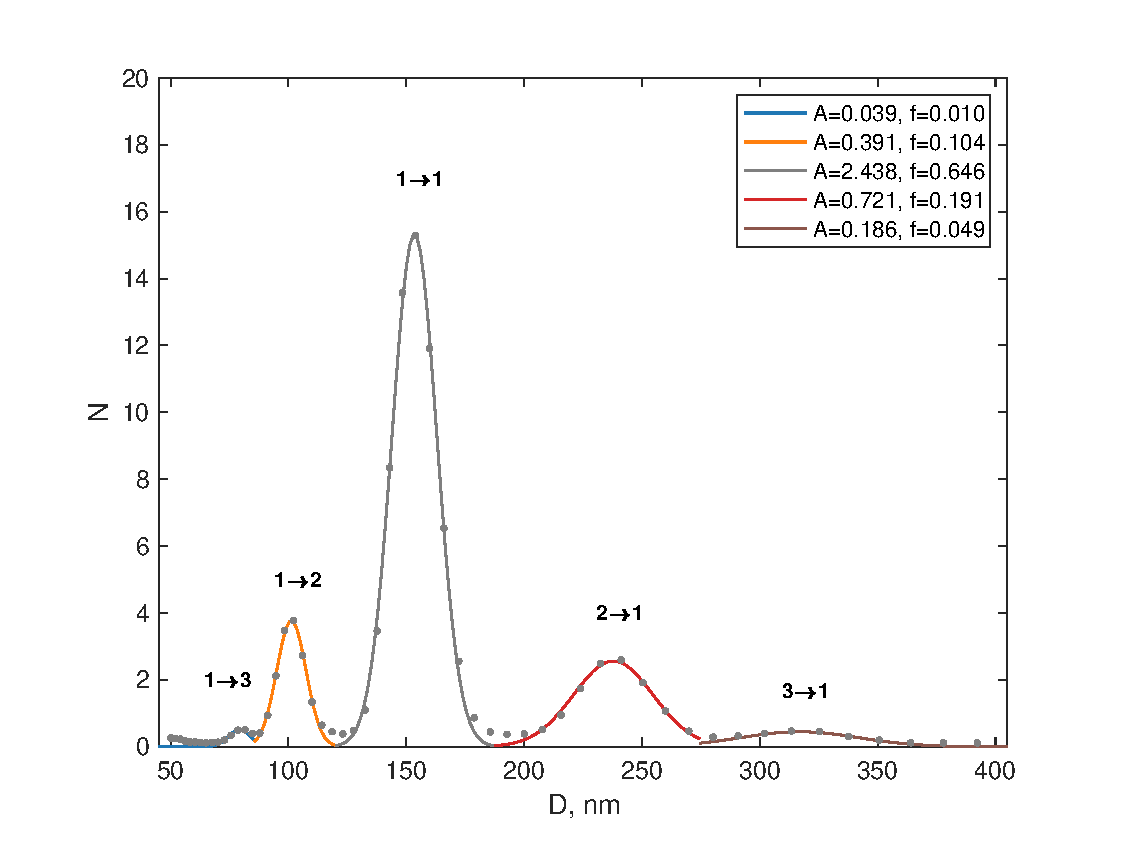
\includegraphics[scale=0.7]{images/fig_supp_recharged_nigrosin.eps}
\caption{Recharged TDMA scan of 150 nm nigrosin particles. Labels above peaks indicate the charging history of the particles, e.g., $2\rightarrow$1 corresponds to the 236 nm particles that acquired two charges in the first diffusion charger, were size classified by DMA1 as 150 nm particles, became singly charged after passing through the second diffusion charger, and then were size classified as 236 nm particles by DMA2.}
\label{s:fig:tdma}
\end{figure}

To quantify the number fraction of doubly charged particles, each mode on the recharged TDMA scan was fitted to a Gaussian probability density function with an added scaling factor. Fit function for an $N$-modal distribution:

\begin{equation}
    \phi(D)=\sum_{i=1}^{N}{\phi_i(D)}=\sum_{i=1}^{N}{\frac{a_i}{\sigma_i\sqrt{2\pi}}e^{-\frac{1}{2}\left(\frac{D-\mu_i}{\sigma_i}\right)^2}}
    \label{s:eq:gaussian-mode}
\end{equation}

\noindent To find the number fractions corresponding to each mode, the area under the respective curve needs to be calculated:

\begin{equation}
    \int_{-\infty}^\infty{\phi_i(D)dD}=a_i
\end{equation}

\noindent The number fraction corresponding to each mode is the ratio of its area to the sum of areas of all modes:

\begin{equation}
    f_n=\frac{a_n}{\sum_{i=1}^{N}{a_i}}
    \label{s:eq:gaussian-fraction}
\end{equation}

\noindent Figure \ref{s:fig:recharged_all} shows recharged TDMA scans for all types of particles considered in this study.

\begin{figure}
	\resizebox{\textwidth}{!}{
		\begin{tikzpicture}
			\begin{axis}[
				xlabel=$D/D_0$,
				ylabel=$N$	
			]
                    \addplot+[smooth,no markers] table [x=X_150,y=Y_150,col sep=comma]{plots/tdma_recharged/recharged_soot.csv};
				\addplot+[smooth,no markers,dashed,style={ultra thick}] table [x=X_240,y=Y_240,col sep=comma] {plots/tdma_recharged/recharged_soot.csv};
				\addlegendentry{150 nm}
				\addlegendentry{240 nm}
				\node[anchor=north west] at (rel axis cs:0,1) {\textbf{(a)}};
			\end{axis}
		\end{tikzpicture}
	
		\begin{tikzpicture}
			\begin{axis}[
				xlabel=$D/D_0$,
				ylabel=$N$	
			]
				\addplot+[smooth,no markers] table [x=X_150,y=Y_150,col sep=comma] {plots/tdma_recharged/recharged_nigrosin.csv};
				\node[anchor=north west] at (rel axis cs:0,1) {\textbf{(b)}};
			\end{axis}
		\end{tikzpicture}
	}

	\resizebox{\textwidth}{!}{
		\begin{tikzpicture}
			\begin{axis}[
				xlabel=$D/D_0$,
				ylabel=$N$	
			]
				\addplot+[smooth,no markers] table [x=X_150,y=Y_150,col sep=comma] {plots/tdma_recharged/recharged_cb_cmp.csv};
				\addplot+[smooth,no markers,dashed,style={ultra thick}] table [x=X_240,y=Y_240,col sep=comma] {plots/tdma_recharged/recharged_cb_cmp.csv};
				\addlegendentry{150 nm}
				\addlegendentry{240 nm}
				\node[anchor=north west] at (rel axis cs:0,1) {\textbf{(c)}};
			\end{axis}
		\end{tikzpicture}
		
		\begin{tikzpicture}
			\begin{axis}[
				xlabel=$D/D_0$,
				ylabel=$N$	
			]
				\addplot+[smooth,no markers] table [x=X_150,y=Y_150,col sep=comma] {plots/tdma_recharged/recharged_cb_agg.csv};
				\addplot+[smooth,no markers,dashed,style={ultra thick}] table [x=X_240,y=Y_240,col sep=comma] {plots/tdma_recharged/recharged_cb_agg.csv};
				\addlegendentry{150 nm}
				\addlegendentry{240 nm}
				\node[anchor=north west] at (rel axis cs:0,1) {\textbf{(d)}};
			\end{axis}
		\end{tikzpicture}
	}
	\caption{TDMA scans of recharged aerosols: (a) soot, (b) nigrosin, $D_0=150\ \mathrm{nm}$, (c) compact CB, and (d) agglomerated CB}
 \label{s:fig:recharged_all}
\end{figure}

\subsection{Effect of multiple charging on particle mass measurements}
\label{s:sec:multiple_charging_and_mass}

The relationship in Equation \ref{s:eq:mult_charging} is used to determine the effective mass of multiply charged particles that is the mass that will be measured by the APM. The apparent mass is lower than the true mass by a factor of $n_1$/$n_2$.

\begin{equation}
    \label{s:eq:mult_charging}
    \frac{m_2}{m_1}=\frac{n_1}{n_2}\left(\frac{D_2}{D_1}\right)^\varepsilon
\end{equation}


\noindent In equation \ref{s:eq:mult_charging}, $m_1$ and $m_2$ are the apparent masses of particles carrying $n_1$ and $n_2$ elementary charges, $D_1$ and $D_2$ are the electrical mobility diameters of the particles, and $\varepsilon$ is the mass-mobility exponent. Note that $\varepsilon = 3$ for spherical particles and $\varepsilon > 1$ for non-spherical particles, which accounts for the variation of effective density of such particles with size.

\begin{table}[ht]
\caption{Electrical mobility diameters and masses of singly and doubly charged particles}
\label{s:tab:double_charges}
\begin{center}
\begin{tabular}{ c c c c } 
 \hline
 $D_1$, nm & $D_2$, nm & $D_2/D_1$ & $m_2/m_1$\tablefootnote{$m_2/m_1=0.5\times (D_2/D_1)^3$; the multiplier $0.5$ accounts for the presence of two charges on particles with mass $m_2$. These mass ratios assume an $\varepsilon$ of 3 and are not applicable to all types of particles} \\
 \hline
150 & 236 & 1.57 & 1.95\\
240 & 397 & 1.66 & 2.27\\
350 & 603 & 1.72 & 2.56\\
 \hline
\end{tabular}
\end{center}
\end{table}

\noindent As seen in Table \ref{s:tab:double_charges}, spherical doubly charged particles of the same electrical mobility diameter as singly charged particles have their apparent mass approximately twice the mass of singly charged particles on an APM scan. Hence, in some cases these doubly charged particles can contribute to the right shoulder of the main mass distribution, biasing the mean mass high. For each $D_1$, the fraction of doubly charged particles can be estimated based on total aerosol size distribution and charging probability \citep{RN10}. The fact that PSL produced the mass-mobility exponent of 3.00 supports this hypothesis, since for PSL spheres, which are truly monodisperse in suspension, doubly charged particles are discarded by DMA during mobility classification.
% The impact of multiple charging on the mass-mobility exponent was estimated from size distribution of nigrosin and charging probabilities and results are available  in supplemental information (Table S, Figure S, Text S?).

% \begin{figure}[htp]
% \centering
% 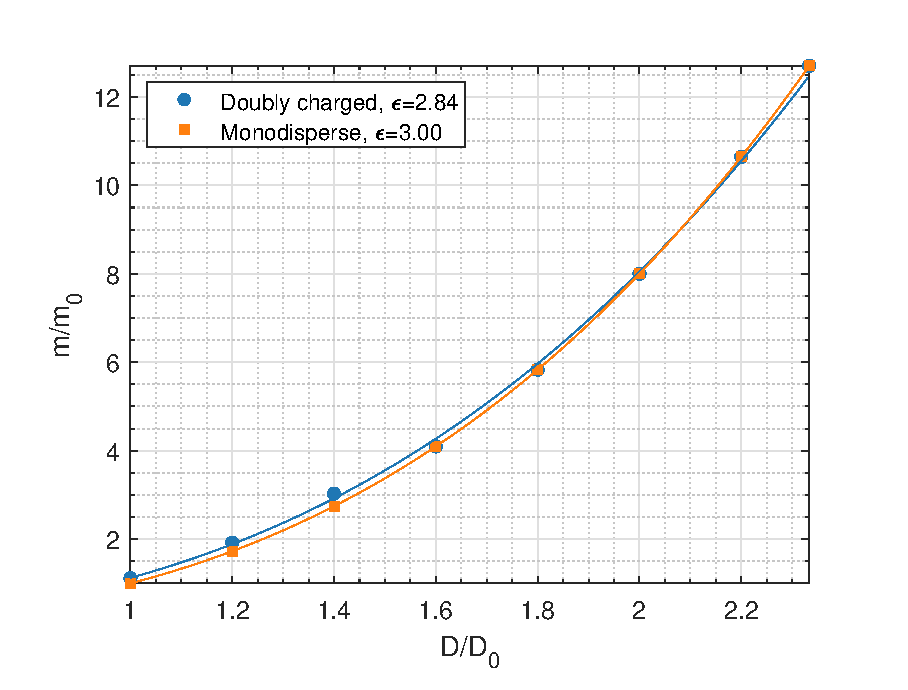
\includegraphics[scale=0.7]{images/fig_supp_mult_charged_nigrosin.eps}
% \caption{Mass of bare aerosol in femtograms vs mobility diameter in nanometers}
% \label{s:fig:mult_nigrosin}
% \end{figure}

% \begin{figure}[htp]
% \centering
% 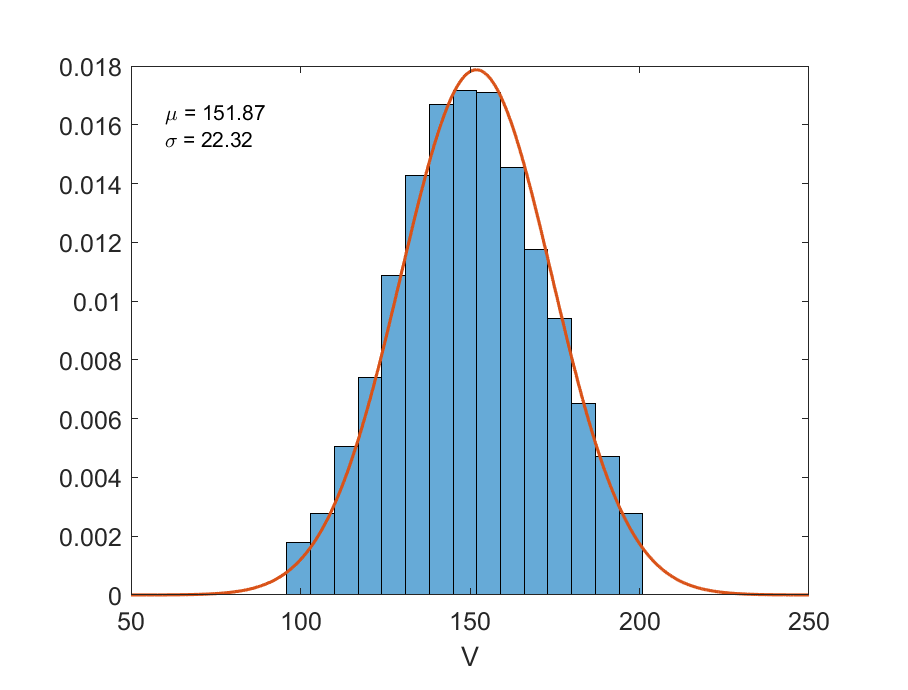
\includegraphics[scale=0.7]{images/fig_supp_apm.eps}
% \caption{Mass of bare aerosol in femtograms vs mobility diameter in nanometers}
% \label{s:fig:apm}
% \end{figure}

\section{Morphology}
% Mass-mobility data that was used to create Figure \ref{fig:mass_mobility} is presented in Figure \ref{s:fig:mass_mobility} in its absolute form.

% \begin{figure}[htp]
% \centering
% 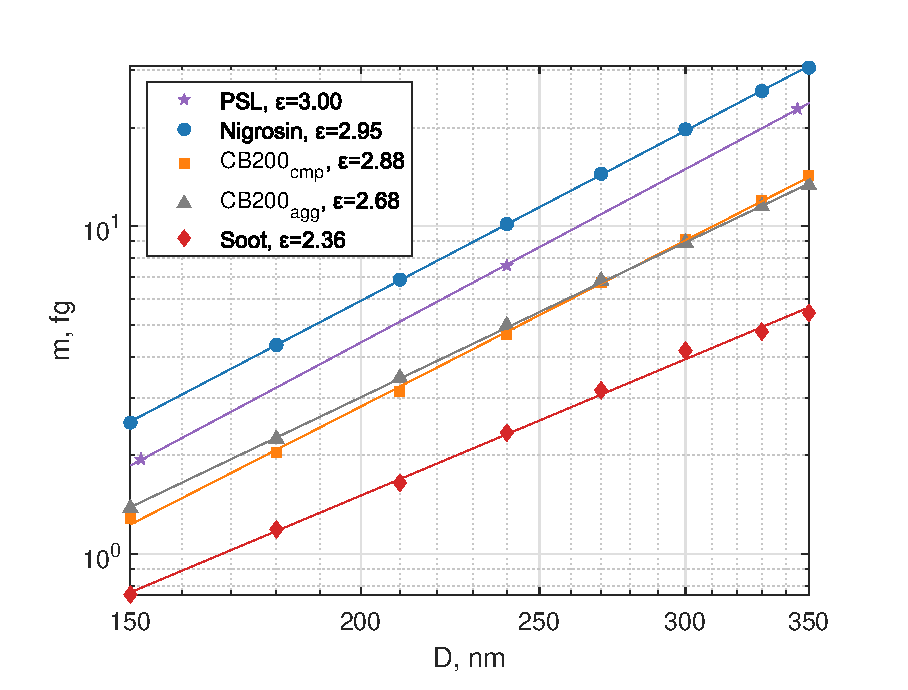
\includegraphics[scale=0.7]{images/fig_supp_mass_mobility.eps}
% \caption{Mass of bare aerosol in femtograms vs mobility diameter in nanometers}
% \label{s:fig:mass_mobility}
% \end{figure}

Relationship between the mass growth factor ($\rm Gfm$) and volume-equivalent coating thickness ($\Delta r_{ve}$) is presented in Figure \ref{s:fig:drve}. The conversion can be performed with Equation \ref{eq:drve} from main text.

\begin{figure}[htp]
\centering
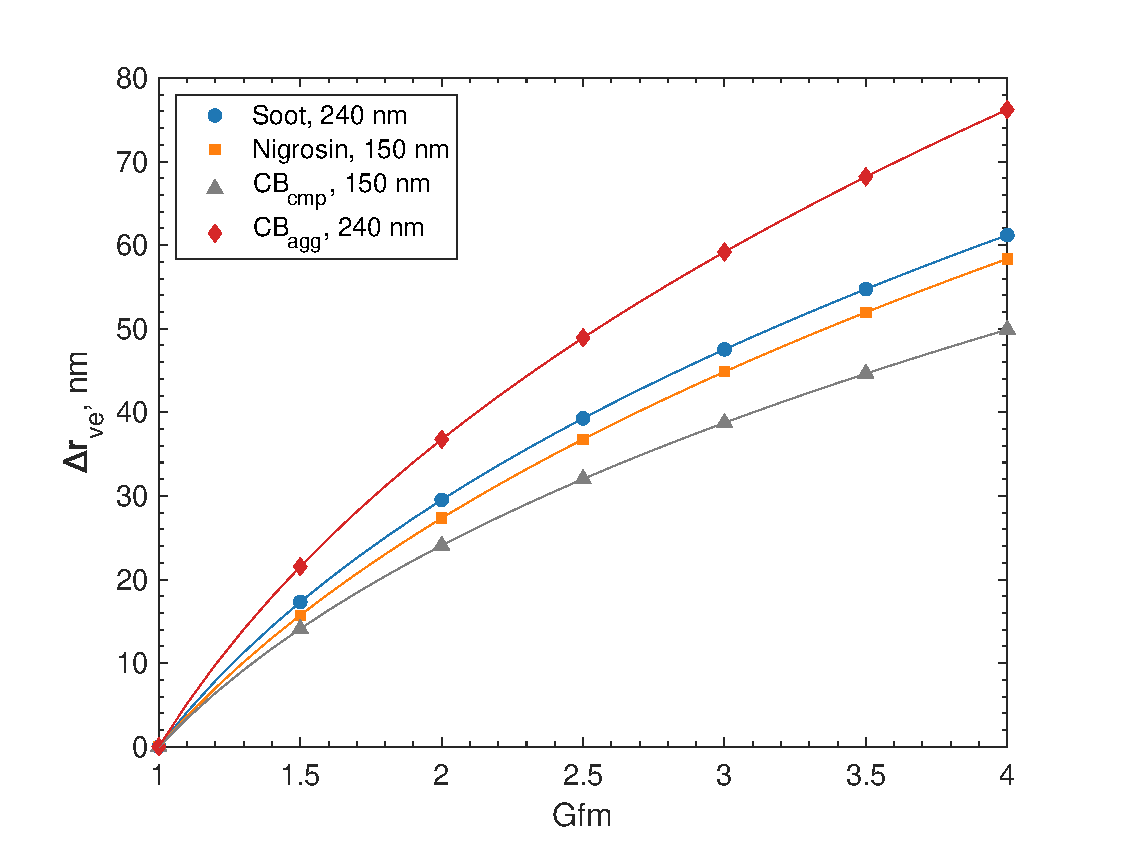
\includegraphics[scale=0.7]{images/fig_supp_drve.eps}
\caption{Volume equivalent coating thickness vs mass growth factor (markers at every 5\textsuperscript{th} point)}
\label{s:fig:drve}
\end{figure}

\section{Absolute cross sections: experiment, Mie, and DDA}
% \subsection{Single scattering albedo}

% A parameter frequently used by climate modelers is single scattering albedo (SSA), which is defined as the ratio of scattering to extinction. This property helps quantify is a particle is a climate warmer of cooler due to prevailing absorption or scattering. If SSA is lower than ½, then most of attenuated light is absorbed and the particle is a warming agent and vice versa. Figure \ref{s:fig:ssa} reports measured SSA values for ($a$) coated and ($b$) coated-denuded particles. It shows that aging makes aerosols better coolers since scattering increases more than absorption.

% \begin{figure}[htp]
% \centering
% 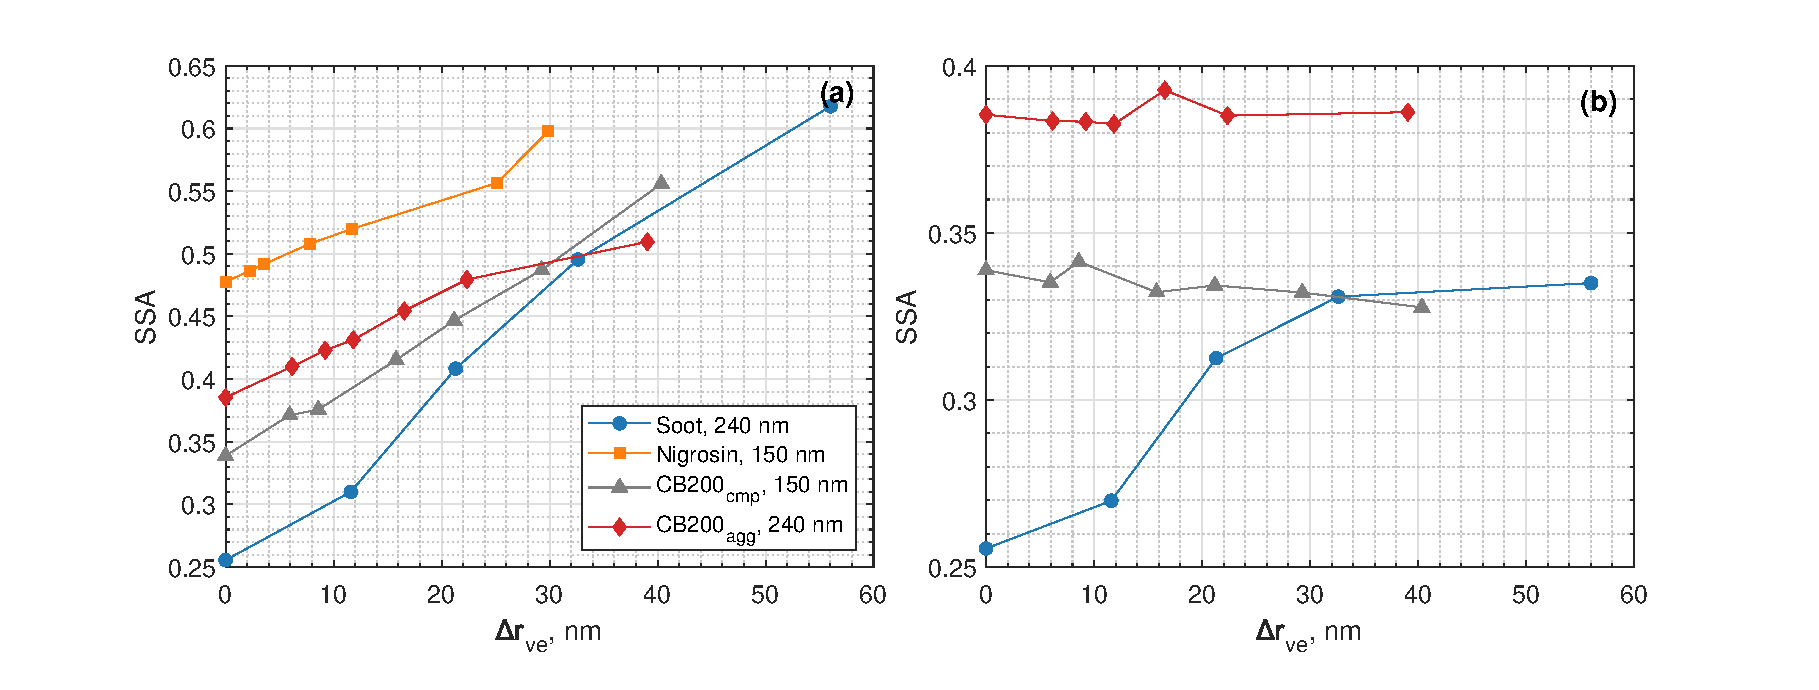
\includegraphics[width=\textwidth]{images/fig_supp_ssa.eps}
% \caption{Single scattering albedo of coated aerosols versus volume equivalent coating thickness}
% \label{s:fig:ssa}
% \end{figure}

Absorption and scattering cross sections that were used to calculate enhancements for Figures \ref{fig:mie_abs} and \ref{fig:mie_sca} are reported in their absolute form in Figures \ref{s:fig:mie_abs} and \ref{s:fig:mie_sca}. Modeled scattering and absorption cross sections that were used to calculate optical enhancements for Figure \ref{fig:dda} are reported in their absolute form in Figure \ref{s:fig:dda}.

\begin{figure}[htp]
    \centering
    \resizebox{\columnwidth}{!}{\begin{tikzpicture}
    \begin{axis}[
    xlabel={$\Delta r_\mathrm{ve},\ \mathrm{nm}$},
    ylabel={$C_\mathrm{abs},\ \mathrm{\mu m}^2$},
    legend pos=north west,
    legend cell align={left},
    ymin=1.0e-2,
    ymax=4.5e-2
    ]
        \addplot [only marks,color=tab_blue,mark=otimes*,error bars/.cd, y dir=both, y explicit] table [col sep=tab,y=C_abs,y error=C_abs_err] {plots/absolute_experimental/soot_coated.txt};
        \addlegendentry{Experimental}
        \addplot [no markers,color=tab_blue] table [col sep=tab,y=C_abs_mie] {plots/absolute_mie/soot.txt};
        \addlegendentry{Mie(+)}
        \addplot [ultra thick,dashed,no markers,color=tab_blue] table [col sep=tab,y=C_abs_corr] {plots/absolute_mie/soot.txt};
        \addlegendentry{Mie(++)}
        \addplot [ultra thick,dotted,no markers,color=tab_blue] table [col sep=tab,y=C_abs_rdg] {plots/absolute_mie/soot.txt};
        \addlegendentry{RDG/Mie}
        \node[anchor=north east] at (rel axis cs:1,1) {\textbf{(a)}};
        \node[anchor=south east] at (rel axis cs:1,0) {\textbf{BC}};
    \end{axis}
    \end{tikzpicture}
    \begin{tikzpicture}
    \begin{axis}[
    xlabel={$\Delta r_\mathrm{ve},\ \mathrm{nm}$},
    ylabel={$C_\mathrm{abs},\ \mathrm{\mu m}^2$},
    legend pos=north west,
    legend cell align={left},
    ymin=1.0e-2,
    ymax=4.5e-2
    ]
        \addplot [only marks,color=tab_orange,mark=square*] table [col sep=tab,y=C_abs] {plots/absolute_experimental/nigrosin.txt};
        \addlegendentry{Experimental}
        \addplot [no markers,color=tab_orange] table [col sep=tab,y=C_abs_mie] {plots/absolute_mie/nigrosin.txt};
        \addlegendentry{Mie(+)}
        \addplot [ultra thick,dashed,no markers,color=tab_orange] table [col sep=tab,y=C_abs_corr] {plots/absolute_mie/nigrosin.txt};
        \addlegendentry{Mie(++)}
        \node[anchor=north east] at (rel axis cs:1,1) {\textbf{(b)}};
        \node[anchor=south east] at (rel axis cs:1,0) {\textbf{Nigrosin}};
    \end{axis}
    \end{tikzpicture}}
    \resizebox{\columnwidth}{!}{\begin{tikzpicture}
    \begin{axis}[
    xlabel={$\Delta r_\mathrm{ve},\ \mathrm{nm}$},
    ylabel={$C_\mathrm{abs},\ \mathrm{\mu m}^2$},
    legend pos=north west,
    legend cell align={left},
    ymin=0.2e-2,
    ymax=7.5e-2
    ]
        \addplot [only marks,color=tab_grey,mark=triangle*] table [col sep=tab,y=C_abs] {plots/absolute_experimental/cb_cmp_coated.txt};
        \addlegendentry{Experimental}
        \addplot [no markers,color=tab_grey] table [col sep=tab,y=C_abs_mie] {plots/absolute_mie/cb_cmp.txt};
        \addlegendentry{Mie(+)}
        \addplot [ultra thick,dashed,no markers,color=tab_grey] table [col sep=tab,y=C_abs_corr] {plots/absolute_mie/cb_cmp.txt};
        \addlegendentry{Mie(++)}
        \addplot [ultra thick,dotted,no markers,color=tab_grey] table [col sep=tab,y=C_abs_rdg] {plots/absolute_mie/cb_cmp.txt};
        \addlegendentry{RDG/Mie}
        \node[anchor=north east] at (rel axis cs:1,1) {\textbf{(c)}};
        \node[anchor=south east] at (rel axis cs:1,0) {\textbf{CB\textsubscript{cmp}}};
    \end{axis}
    \end{tikzpicture}
    \begin{tikzpicture}
    \begin{axis}[
    xlabel={$\Delta r_\mathrm{ve},\ \mathrm{nm}$},
    ylabel={$C_\mathrm{abs},\ \mathrm{\mu m}^2$},
    legend pos=north west,
    legend cell align={left},
    ymin=2.5e-2,
    ymax=6.5e-2
    ]
        \addplot [only marks,color=tab_red,mark=diamond*] table [col sep=tab,y=C_abs] {plots/absolute_experimental/cb_agg_coated.txt};
        \addlegendentry{Experimental}
        \addplot [no markers,color=tab_red] table [col sep=tab,y=C_abs_mie] {plots/absolute_mie/cb_agg.txt};
        \addlegendentry{Mie(+)}
        \addplot [ultra thick,dashed,no markers,color=tab_red] table [col sep=tab,y=C_abs_corr] {plots/absolute_mie/cb_agg.txt};
        \addlegendentry{Mie(++)}
        \addplot [ultra thick,dotted,no markers,color=tab_red] table [col sep=tab,y=C_abs_rdg] {plots/absolute_mie/cb_agg.txt};
        \addlegendentry{RDG/Mie}
        \node[anchor=north east] at (rel axis cs:1,1) {\textbf{(d)}};
        \node[anchor=south east] at (rel axis cs:1,0) {\textbf{CB\textsubscript{agg}}};
    \end{axis}
    \end{tikzpicture}}
    \caption{Measured and calculated absorption cross sections for (a) compact soot, (b) nigrosin, (c) compact CB, and (d) agglomerated CB.
    %----were cases c and d swapped for RDG-Mie?
    Measured (markers), calculated with core-shell Mie theory (solid line), and calculated with Mie by accounting for doubly charged particles (dashed line). For cases (a) and (d), the dashed and solid line overlap due to a negligible fraction of double charged particles. Volume equivalent and mobility diameters for each aerosol type are shown in Table \ref{tab:densities}.}
    \label{s:fig:mie_abs}
\end{figure}

\begin{figure}[htp]
    \centering
    \resizebox{\columnwidth}{!}{\begin{tikzpicture}
    \begin{axis}[
    xlabel={$\Delta r_\mathrm{ve},\ \mathrm{nm}$},
    ylabel={$C_\mathrm{sca},\ \mathrm{\mu m}^2$},
    legend pos=north west,
    legend cell align={left},
    ymin=0,
    ymax=6.5e-2
    ]
        \addplot [only marks,color=tab_blue,mark=otimes*] table [col sep=tab,y=C_sca] {plots/absolute_experimental/soot_coated.txt};
        \addlegendentry{Experimental}
        \addplot [no markers,color=tab_blue] table [col sep=tab,y=C_sca_mie] {plots/absolute_mie/soot.txt};
        \addlegendentry{Mie(+)}
        \addplot [ultra thick,dashed,no markers,color=tab_blue] table [col sep=tab,y=C_sca_corr] {plots/absolute_mie/soot.txt};
        \addlegendentry{Mie(++)}
        \node[anchor=north east] at (rel axis cs:1,1) {\textbf{(a)}};
        \node[anchor=south east] at (rel axis cs:1,0) {\textbf{BC}};
    \end{axis}
    \end{tikzpicture}
    \begin{tikzpicture}
    \begin{axis}[
    xlabel={$\Delta r_\mathrm{ve},\ \mathrm{nm}$},
    ylabel={$C_\mathrm{sca},\ \mathrm{\mu m}^2$},
    legend pos=north west,
    legend cell align={left},
    ymin=0,
    ymax=6.5e-2
    ]
        \addplot [only marks,color=tab_orange,mark=square*] table [col sep=tab,y=C_sca] {plots/absolute_experimental/nigrosin.txt};
        \addlegendentry{Experimental}
        \addplot [no markers,color=tab_orange] table [col sep=tab,y=C_sca_mie] {plots/absolute_mie/nigrosin.txt};
        \addlegendentry{Mie(+)}
        \addplot [ultra thick,dashed,no markers,color=tab_orange] table [col sep=tab,y=C_sca_corr] {plots/absolute_mie/nigrosin.txt};
        \addlegendentry{Mie(++)}
        \node[anchor=north east] at (rel axis cs:1,1) {\textbf{(b)}};
        \node[anchor=south east] at (rel axis cs:1,0) {\textbf{Nigrosin}};
    \end{axis}
    \end{tikzpicture}}
    \resizebox{\columnwidth}{!}{\begin{tikzpicture}
    \begin{axis}[
    xlabel={$\Delta r_\mathrm{ve},\ \mathrm{nm}$},
    ylabel={$C_\mathrm{sca},\ \mathrm{\mu m}^2$},
    legend pos=north west,
    legend cell align={left},
    ymin=0,
    ymax=3.5e-2
    ]
        \addplot [only marks,color=tab_grey,mark=triangle*] table [col sep=tab,y=C_sca] {plots/absolute_experimental/cb_cmp_coated.txt};
        \addlegendentry{Experimental}
        \addplot [no markers,color=tab_grey] table [col sep=tab,y=C_sca_mie] {plots/absolute_mie/cb_cmp.txt};
        \addlegendentry{Mie(+)}
        \addplot [ultra thick,dashed,no markers,color=tab_grey] table [col sep=tab,y=C_sca_corr] {plots/absolute_mie/cb_cmp.txt};
        \addlegendentry{Mie(++)}
        \node[anchor=north east] at (rel axis cs:1,1) {\textbf{(c)}};
        \node[anchor=south east] at (rel axis cs:1,0) {\textbf{CB\textsubscript{cmp}}};
    \end{axis}
    \end{tikzpicture}
    \begin{tikzpicture}
    \begin{axis}[
    xlabel={$\Delta r_\mathrm{ve},\ \mathrm{nm}$},
    ylabel={$C_\mathrm{sca},\ \mathrm{\mu m}^2$},
    legend pos=north west,
    legend cell align={left},
    ymin=0,
    ymax=6.5e-2
    ]
        \addplot [only marks,color=tab_red,mark=diamond*] table [col sep=tab,y=C_sca] {plots/absolute_experimental/cb_agg_coated.txt};
        \addlegendentry{Experimental}
        \addplot [no markers,color=tab_red] table [col sep=tab,y=C_sca_mie] {plots/absolute_mie/cb_agg.txt};
        \addlegendentry{Mie(+)}
        \addplot [ultra thick,dashed,no markers,color=tab_red] table [col sep=tab,y=C_sca_corr] {plots/absolute_mie/cb_agg.txt};
        \addlegendentry{Mie(++)}
        \node[anchor=north east] at (rel axis cs:1,1) {\textbf{(d)}};
        \node[anchor=south east] at (rel axis cs:1,0) {\textbf{CB\textsubscript{agg}}};
    \end{axis}
    \end{tikzpicture}}
    \caption{Measured and calculated scattering cross sections for (a) compact soot, (b) nigrosin, (c) compact CB, and (d) agglomerated CB. Measured (markers), calculated with core-shell Mie theory (solid line), and calculated with Mie by accounting for doubly charged particles (dashed line). For cases (a) and (d), the dashed and solid line overlap due to a negligible fraction of double charged particles. Volume equivalent and mobility diameters for each aerosol type are shown in Table \ref{tab:densities}.}
    \label{s:fig:mie_sca}
\end{figure}

\begin{figure}[htp]
\centering
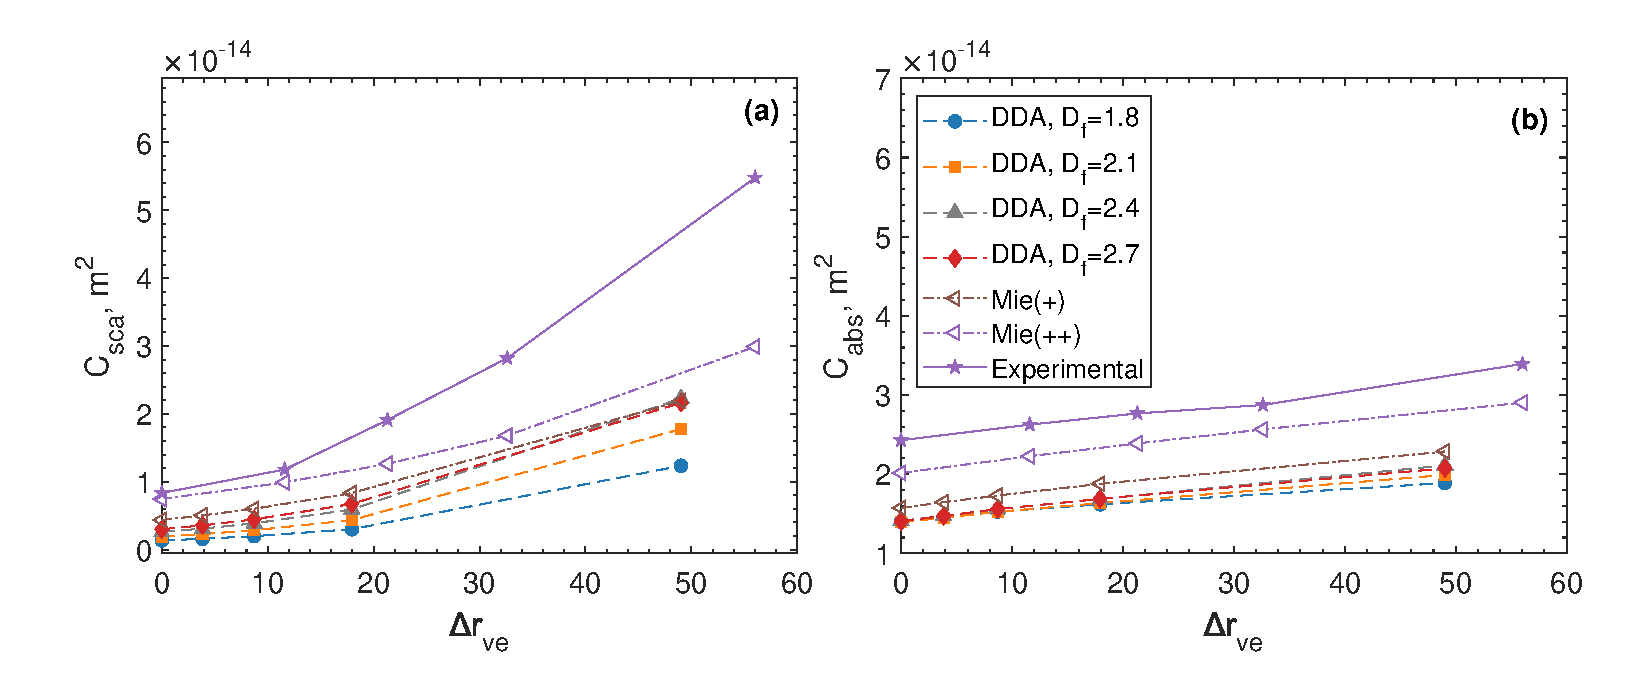
\includegraphics[width=\textwidth]{images/absolute-optics-modeling.eps}
\caption{Experimentally measured and computed (Mie and DDA) scattering and absorption cross sections for DOS-coated soot}
\label{s:fig:dda}
\end{figure}

\section{Fractal dimension of coated-denuded soot}
\label{s:sec:drve2df}

DDA was used to calculate scattering enhancements for coated-denuded soot. Since the parameter that changes with coating thickness for coated-denuded soot is compactness, the optical calculations were performed for several aggregates with fractal dimensions ranging from 1.8 to 2.7. To map experimental data to calculated values, we used an exponential decay function to relate coating thickness and fractal dimension:

\begin{equation}
    D_f=2.8-(2.8-1.8)\cdot e^{-\frac{\Delta r_{ve}}{a}}
\end{equation}

\begin{equation}
    a=-\frac{\Delta r_{ve,max}}{\ln{\frac{2.8-2.7}{2.8-1.8}}}
\end{equation}

\section{Coating thickness of multiply charged particles}
\label{s:sec:drve_multiply_charged}

In this section, we derive an equation that relates the coating thicknesses of singly and doubly charged particles. For a spherical particle, the rate of condensation is inversely proportional to particle radius \citep{RN2},

\begin{equation}
    \frac{dr}{dt}=\left(C-C_{s,Kelvin}\right)C_{FS}D_iM\frac{1}{\rho r}
    \label{s:eq:condensation}
\end{equation}

\noindent where $C$ is the vapor concentration, $C_{s,Kelvin}$ is the Kelvin-corrected saturated vapor concentration, $C_{FS}$ is the transition regime correction factor, $D_i$ is the gas diffusivity of the coating material, $M$ is the molar mass of the coating material, $\rho$ is the material mass density of the coating material, and $r$ the is particle radius. The continuum regime equation with a transition correction factor was selected because the size of particles used in this study is greater than the mean free path of air. If we assume that supersaturation produced by the coating chamber is high enough that Kelvin effect can be neglected and $C_{FS}$ does not change significantly between singly and doubly charged particles (mobility diameter differs by a factor of approximately 1.5), equation \ref{s:eq:condensation} can be written as,

\begin{equation}
    \frac{dr}{dt}=A\frac{1}{r}
\end{equation}

\noindent where $A$ is some constant. The differential equation can then be solved by separation of variables,

\begin{equation}
    r^2=2At+r_i^2
\end{equation}

\noindent where $r_i$ is the radius of a bare particle. With the assumptions made, the quantity $2At$ is independent of particle size. We can now write equation for particles of different sizes - singly charged particle of initial radius $r_{i1}$ and doubly charged particle of radius $r_{i2}$. Additionally, $r_1$ can be expressed as $r_{i1}+\Delta r_1$, where $\Delta r_1$ is coating thickness of the singly charged particle. Then we can solve for $2At$ in terms of $r_{i1}$ and $\Delta r_1$ and plug the expression into the equation for $\Delta r_2$.

\begin{equation}
    \Delta r_2=\sqrt{\Delta r_1\left(2r_{i1}+\Delta r_1\right)+r_{i2}^2}-r_{i2}
    \label{s:eq:thickness}
\end{equation}

\begin{figure}[htp]
\centering
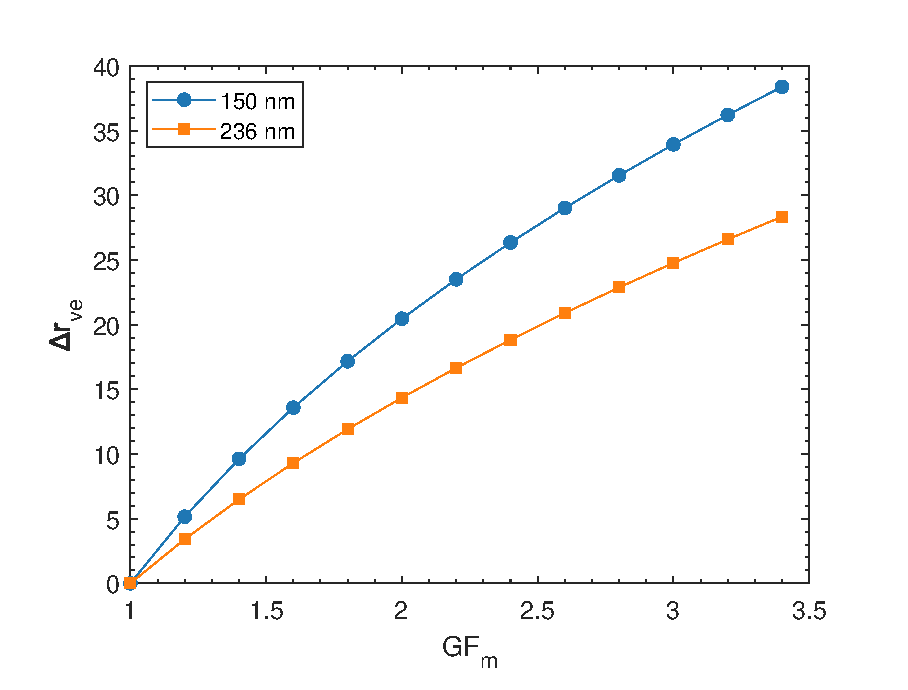
\includegraphics[scale=0.7]{images/fig_supp_thickness_formula.eps}
\caption{Volume equivalent coating thickness of singly charged compact CB particles (measured) and doubly charged compact CB particles (calculated using equation \ref{s:eq:thickness}) versus Gfm of singly charged particles.}
\label{s:fig:thickness}
\end{figure}

Figure \ref{s:fig:thickness} shows the change in volume equivalent coating thickness of 150 nm compact CB, which was measured experimentally, and coating thickness of doubly charged particles with initial mobility diameter of 236 nm calculated with equation \ref{s:eq:thickness}. Coating thickness of larger particles is consistently lower than that of smaller particles.

To account for the slower diameter growth of doubly charged particles in optical calculations, for each particle type, two datasets of optical cross sections were calculated with Mie: one for smaller singly charged particles with coating thicknesses obtained experimentally and one for larger doubly charged particles with coating thicknesses calculated with Equation \ref{s:eq:thickness}. A number-weighted average ($C_{avg}$) between these datasets was calculated at each point,

\begin{equation}
    C_{avg}=f_1C_1+f_2C_2
\end{equation}

\noindent where $f_1$ is number fraction of singly charged particles, $C_1$ is optical cross section of singly charged particles, $f_2$ is number fraction of doubly charged particles, and $C_2$ is optical cross section of doubly charged particles. These corrected cross sections are also reported in Figures \ref{fig:mie_sca} and \ref{fig:mie_abs}.



% Processed images go here

\section{Effect of different refractive indices of soot and its surrogates}

The choice of refractive index for a material may have a significant effect on the outcome of optical calculations. Similarly, the difference in complex refractive indices between soot and its surrogates can contribute to different optical responses during particle processing. Being the same material chemically, CB and mature soot are expected to have similar refractive indices. However, the imaginary part of the complex refractive index of nigrosin is significantly lower than that of soot (Table \ref{tab:refindices} in main text). To evaluate the impact of this difference, we calculated $E_{abs}$, $E_{sca}$, and $SSA$ of spherical 150 nm particles made of soot ($1.7+0.6i$) and nigrosin ($1.7+0.3i$) that were coated by DOS ($1.4+0.0i$) (Table \ref{tab:ssa}). Remarkably, the enhancement in light absorption is similar between soot and nigrosin (within $4\%$ for the 40 nm coating thickness), but enhancement in light scattering and SSA are significantly different, by $25\%$ and $32\%$, respectively. Thus, using nigrosin as a surrogate of soot may lead to a significant underestimation of light scattering by coated combustion aerosols.  


%\textcolor{blue}{For aerosols, refractive indices are often retrieved from experimental optical measurements. To carry out a reverse calculation, an optical model needs to be used. \citet{RN67} compare complex refractive indices of soot retrieved by two different optical models: Mie and RDG. At 532 nm wavelength, they found the refractive index of soot to be $1.96+1.01i$ (Mie) and $1.80+1.43i$ (RDG).}

%\textcolor{red}{Note: Also consider adding a brief discussion on model dependence of the complex refractive index of soot. First, use two different indices of soot (e.g., RDG and Mie based from Forestieri) to predict enhancements and SSA, similar as you did in table 5 for soot vs nigrosin. If the difference is significant, e.g., 10 percent or more, then certainly this is worth discussing in a few sentences.}\textcolor{blue}{Added above, but this may raise some questions. The RIs provided by \citet{RN67} are very different from what we used in our calculations}

% SSA for different RIs
\begin{table}[!ht]
    \centering
    \caption{SSA for 150 nm particles with $1.7+0.6i$ (Soot \& CB) and $1.7+0.3i$ (nigrosin) refractive indices coated with DOS calculated using Mie}
    \begin{tabular}{c c c c c c c}
        \hline
        & \multicolumn{2}{c}{SSA} & \multicolumn{2}{c}{$E_\mathrm{abs}$} & \multicolumn{2}{c}{$E_\mathrm{sca}$} \\
        $\Delta r_{\mathrm{ve}},\ \mathrm{nm}$ & $1.7+0.6i$ & $1.7+0.3i$ & $1.7+0.6i$ & $1.7+0.3i$ & $1.7+0.6i$ & $1.7+0.3i$ \\
        \hline
        0 & 0.248 & 0.306 & 1.00 & 1.00 & 1.00 & 1.00\\
        10 & 0.295 & 0.383 & 1.11 & 1.12 & 1.40 & 1.57\\
        20 & 0.345 & 0.460 & 1.20 & 1.22 & 1.92 & 2.37\\
        40 & 0.450 & 0.597 & 1.37 & 1.42 & 3.40 & 4.79\\
        80 & 0.672 & 0.800 & 1.71 & 1.79 & 10.60 & 16.25\\
        \hline
    \end{tabular}
    \label{tab:ssa}
\end{table}


%Necking references:
%\begin{itemize}
%    \item \citet{RN28} - Effects of necking on absorption
%    \item \citet{RN74} - Different neck representations
%\end{itemize}


\bibliographystyle{elsarticle-harv} 
\bibliography{cas-refs}

\end{document}
